%!TEX root=masterproef.tex

\chapter{Simulatie van routering voor een XBee-gebaseerd maasnetwerk}
\label{virtual-mesh}

Het hardwareplatform, beschreven in bijlage \ref{hardware-platform}, beschikt
over een XBee-module om het ZigBee-netwerk op te bouwen. Deze module biedt een
zeer hoogniveau interface aan, waardoor routering en concepten op lagere
niveaus in het algemeen verborgen blijven. Zo is het bv. onmogelijk om
communicatie die niet voor de eigen radio bestemd is op te vangen, terwijl dit
net een typische eigenschap is van een draadloos (maas)netwerk.

Aangezien het kunnen opvolgen van het verder doorsturen van berichten een
belangrijk aspect is in het kader van deze masterproef, en hiervoor alle
communicatie die opgevangen kan worden ter beschikking moet staan van het
algoritme, was het nodig om dit gedrag na te bootsen om een realistische
demonstratie van de algoritmen mogelijk te maken. Hiertoe werd een virtuele
routering ge\"implementeerd.

\section{Broadcasting}
\label{zigbee-broadcasting}

In een eerste fase werd deze virtuele routering gerealiseerd door middel van
\emph{broadcasting}. Hierbij wordt een bericht naar alle knopen in het netwerk
verstuurd. Op deze manier komt een bericht niet alleen toe bij de effectieve
bestemmeling, maar ook bij andere knopen, waardoor het \emph{afluistergedrag}
gesimuleerd kan worden. Door toevoegen van extra informatie over de
oorspronkelijke verzender, de tussenliggende knoop waarlangs de boodschap
verzonden werd en de uiteindelijke bestemmeling, kan een knoop bepalen of een
bericht aan hem verzonden is, of dat het een \emph{afgeluisterde} boodschap is
die verzonden was tussen twee andere knopen.

Deze implementatie was eenvoudig maar doeltreffend, maar ook slechts in theorie
een goede oplossing. In de praktijk bleek dit niet zo te zijn. Het probleem
ontstaat bij de manier waarop \emph{broadcasting} ge\"implementeerd is in het
ZigBee-protocol. Uit de handleiding van de XBee-module \citep{manual:xbee}
leren we immers dat:

\begin{quote}

\emph{Each node that transmits the broadcast will also create an entry in a
local broadcast transmission table. This entry is used to keep track of each
received broadcast packet to ensure the packets are not endlessly transmitted.
Each entry persists for 8 seconds. The broadcast transmission table holds 8
entries.}

\emph{For each broadcast transmission, the ZigBee stack must reserve buffer
space for a copy of the data packet. This copy is used to retransmit the packet
as needed. Large broadcast packets will require more buffer space. This
information on buffer space is provided for general knowledge; the user does
not and cannot change any buffer spacing. Buffer spacing is handled
automatically by the XBee module.}

\emph{Since broadcast transmissions are retransmitted by each device in the
network, broadcast messages should be used sparingly.}

\end{quote}

De \emph{broadcast transmission table} heeft slechts plaats om 8 broadcasts op
te volgen. Elk van die broadcasts moet gedurende 8 seconden bijgehouden worden.
Het is duidelijk dat bij gebruik van broadcasting om alle communicatie te
realiseren, deze buffer snel gevuld is en dat vervolgens pakketten gewoon
verwijderd worden. Dat dit nagenoeg stilzwijgend gebeurt is op zijn minst
bedenkelijk te noemen.

Daarom werd in een tweede implementatie gebruik gemaakt van \emph{unicasting},
of het versturen van een bericht aan \'e\'en specifieke bestemmeling. Bij
\emph{unicasting} kan de bestemmeling een bericht bevestigen, waardoor de
verzender bv. niet gedurende 8 seconden het bericht moet bijhouden. Ook zal,
bij niet-bevestiging door de bestemmeling, tot driemaal toe geprobeerd worden
om het bericht opnieuw te versturen. De garanties omtrent correcte verzending
liggen bij \emph{unicasting} veel hoger.

Dit vraagt echter wel wat meer bijkomend werk, omdat de effecten van
\emph{broadcasting} gesimuleerd moeten worden. Elk bericht dat verstuurd wordt
aan \'e\'en bestemmeling, moet nu ook expliciet naar de overige knopen
verstuurd worden.

\section{Opstelling}

Figuur \ref{fig:xbee-setup} toont de opstelling voor de demonstratie: drie
XBee-modules zijn geconfigureerd als een eindknoop, een router en een
co\"ordinator. De co\"ordinator is via een \emph{explorerboard} verbonden met
een computer. Op deze manier is het mogelijk om deze XBee-module te benaderen
aan de hand van een seri\"ele verbinding. De eindknoop en de router zijn verder
twee identieke sensorknopen.

\begin{figure}[ht]
  \centering
  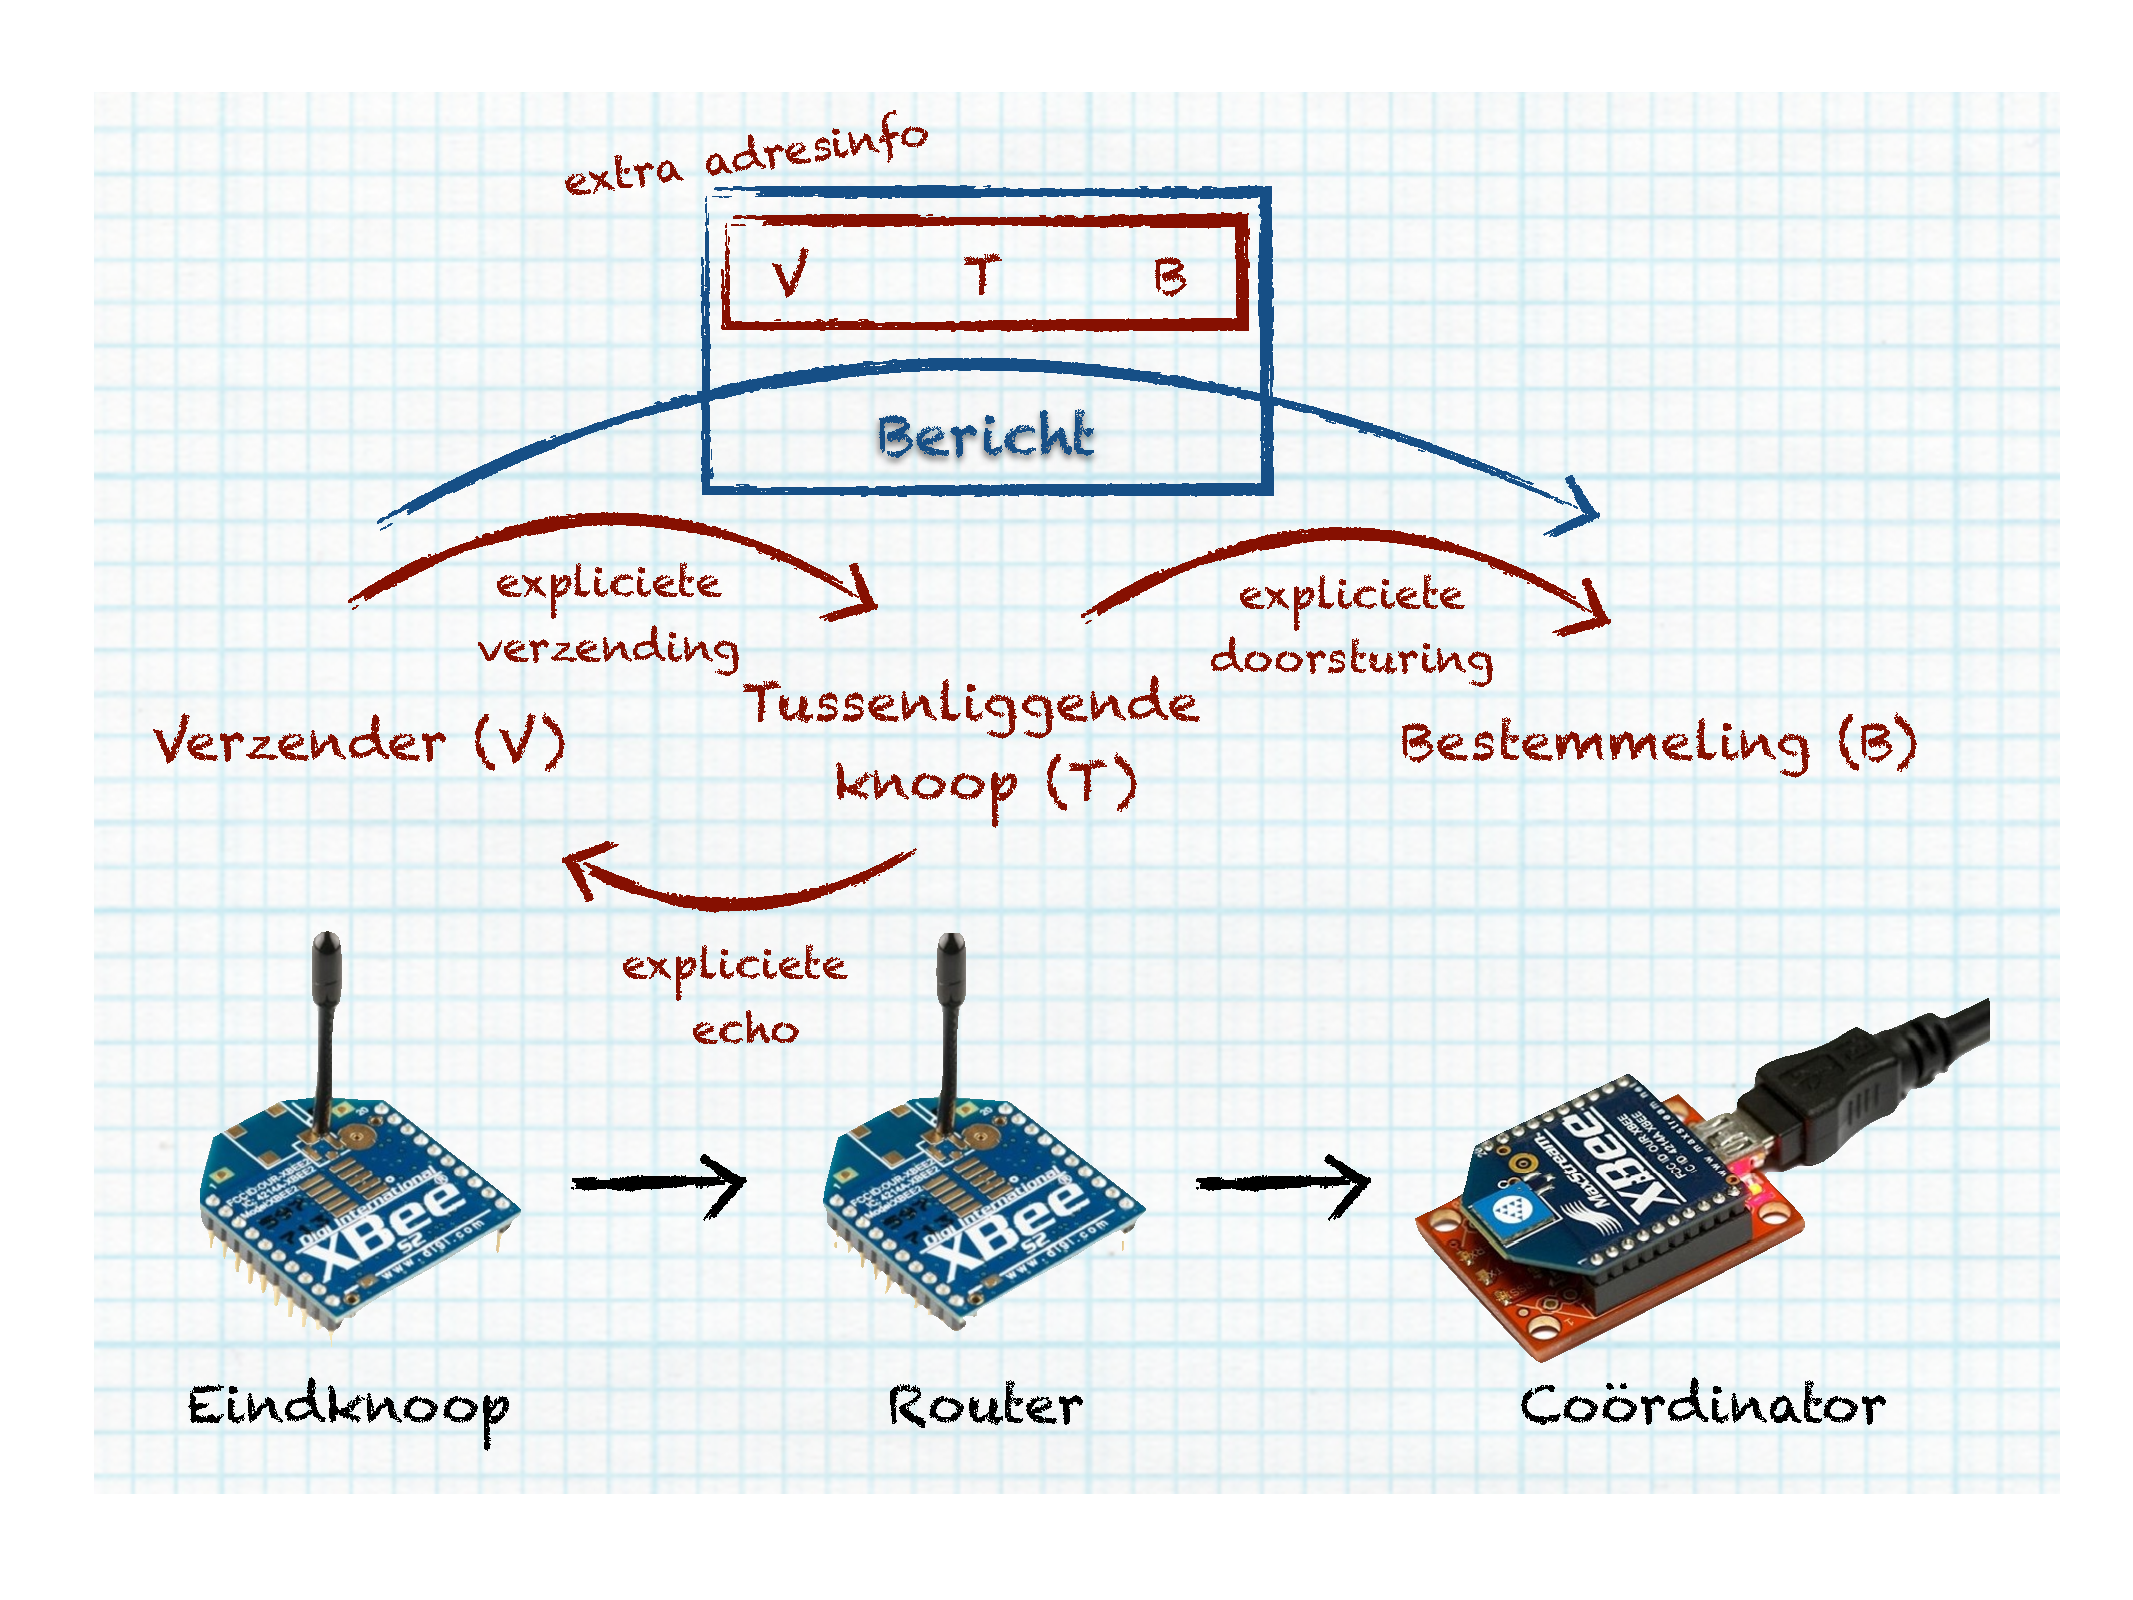
\includegraphics[width=0.9\linewidth]{resources/xbee-setup.pdf}
  \caption{Opstelling van maasnetwerk voor demonstratie}
  \label{fig:xbee-setup}
\end{figure}

Om met de drie XBee-modules op een correcte manier tot een maasnetwerk te
komen, moeten we de modules voorzien van een specifieke configuratie. Zo wordt
bij de co\"ordinator de tijdspanne dat nieuwe knopen het netwerk kunnen
vervoegen beperkt tot \'e\'en minuut. Dit gebeurt aan de hand van het
\emph{Node Join}-commando. Gedurende deze periode kan dan de router geactiveerd
worden. Na associatie van deze radio en het verstrijken van deze minuut, kan de
eindknoop geactiveerd worden. Deze zal niet meer rechtstreeks bij de
co\"ordinator kunnen aansluiten en zal via de router het netwerk moeten
benaderen.

\section{Sturen van berichten}

We kunnen nu onderscheid maken tussen de eindknoop en de router. De eindknoop
wil berichten versturen naar de co\"ordinator en moet hiervoor langs de router
passeren. Het is dus alleen de router die berichten zal moeten doorsturen.
Hierbij zal het bericht niet alleen naar de co\"ordinator verstuurd worden,
maar ook expliciet terug naar de eindknoop. Wanneer de router een bericht
ontvangt, zal hij dit steeds doorsturen naar de co\"ordinator (hijzelf is geen
bestemmeling) en zal hij elk bericht dat hij verstuurt naar de co\"ordinator
(ook zijn eigen berichten) tevens versturen naar de eindknoop. De eindknoop
daarentegen zal nooit berichten voor een andere knoop ontvangen, moet geen
berichten doorsturen en dient daarom ook geen berichten te ontdubbelen.

Bij het versturen van berichten wordt \emph{extra adresinformatie} aan het
bericht toegevoegd, nl. de drie bijkomende netwerkadressen van de betrokken
knopen: het adres van de oorspronkelijke \emph{verzender}, het adres van de
\emph{tussenliggende knoop} en het adres van de uiteindelijke
\emph{bestemmeling}. Aan de hand van deze extra informatie kunnen knopen
bepalen welke rol ze vertolken bij het ontvangen van een bericht en hoe ze er
dus moeten mee omgaan.

De extra code die deze simulatie realiseert is weergegeven in codevoorbeeld
\ref{lst:virtual-mesh}. Ze volgt de opbouw van de overeenkomstige code voor
normale aansturing van de XBee-module: een verzendfunctie, een ontvangfunctie
en de mogelijkheid om een externe functie voor binnenkomende berichten te
registreren.

De werking wordt duidelijk aan de hand van een voorbeeld, waarbij zowel de
eindknoop als de router een bericht verzenden naar de co\"ordinator. De
uitvoer van deze demonstratie is weergegeven in figuren
\ref{fig:virtual-mesh-end-device}, \ref{fig:virtual-mesh-router} en
\ref{fig:virtual-mesh-coordinator}. We zien de uitvoer van respectievelijk de
eindknoop, de router en de co\"ordinator.

Zowel de eindknoop als de router gebruiken exact dezelfde applicatiecode. Na
het initialiseren van de seri\"ele verbinding en het opzetten van de
netwerkassociatie, tonen beide knopen eerst hun eigen netwerkadres en dat van
hun hi\"erarchisch ouderlijke knoop (\emph{parent}). In dit geval heeft de
eindknoop netwerkadres \ttt{ae f5} en de router adres \ttt{fa 7d}. We zien dat
de eindknoop inderdaad de router als \emph{parent} opgeeft.

\inputminted[linenos,frame=lines,framesep=2mm,fontsize=\footnotesize,firstline=97,firstnumber=97]{c}{../src/demo/lib/network.c}
\vspace{-5mm}
\captionof{listing}{Simulatie van een maasnetwerk met XBee modules.
\label{lst:virtual-mesh}}
\vspace{3mm}

\setlength{\parindent}{15pt} % fixes indentation after inputminted

De router geeft als \emph{parent} \ttt{ff fe} aan. Dit adres staat voor een
onbekend adres. XBee routers geven dit adres standaard terug aangezien het
\emph{parent} concept voor hen niet bestaat. In deze beperkte
simulatieopstelling kunnen we dit adres gelijkstellen aan het adres van de
co\"ordinator: \ttt{00 00}.

De router zal na associatie met het netwerk via de co\"ordinator wachten tot er
zich een eindknoop via hem met het netwerk verbindt, alvorens zijn eigen
berichten te versturen. Tijdens het wachten, verwerkt de router wel
binnenkomende berichten. De eindknoop zal tijdens deze opstartfase een (echte)
\emph{broadcast} versturen. Deze \emph{broadcast} bereikt de router die deze
informatie zal gebruiken om de adresgegevens van de eindknoop te bewaren en te
gebruiken om kopies van berichten die hij verzendt ook naar de eindknoop te
sturen. De code van deze opstartfase is weergegeven in codevoorbeeld
\ref{lst:virtual-mesh-init}.

We zien duidelijk dat de berichten van de eindknoop door de router doorgestuurd
worden naar de co\"ordinator. Deze zelfde berichten worden tevens nog een
tweede keer verzonden naar de eindknoop. Zo zien we dat de router twee
berichten ontvangt van de eindknoop en dat de eindknoop er vier ontvangt: twee
van de router zelf en twee doorgestuurde berichten van zichzelf.

\inputminted[linenos,frame=lines,framesep=2mm,fontsize=\footnotesize,firstline=37,lastline=60,firstnumber=37]{c}{../src/demo/lib/network.c}
\vspace{-5mm}
\captionof{listing}{Initialisatie van het maasnetwerk.
\label{lst:virtual-mesh-init}}
\vspace{3mm}

\begin{figure}[ht]
  \centering
  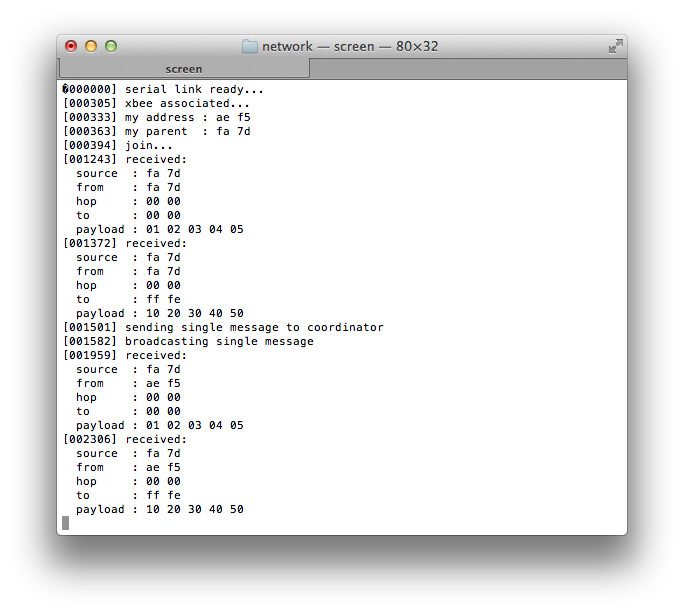
\includegraphics[width=.7\linewidth]{../src/demo/network/end-device.png}
  \vspace{-3mm}
  \caption{Simulatie van een maasnetwerk: Eind-knoop}
  \label{fig:virtual-mesh-end-device}
\end{figure}

\begin{figure}[ht]
  \centering
  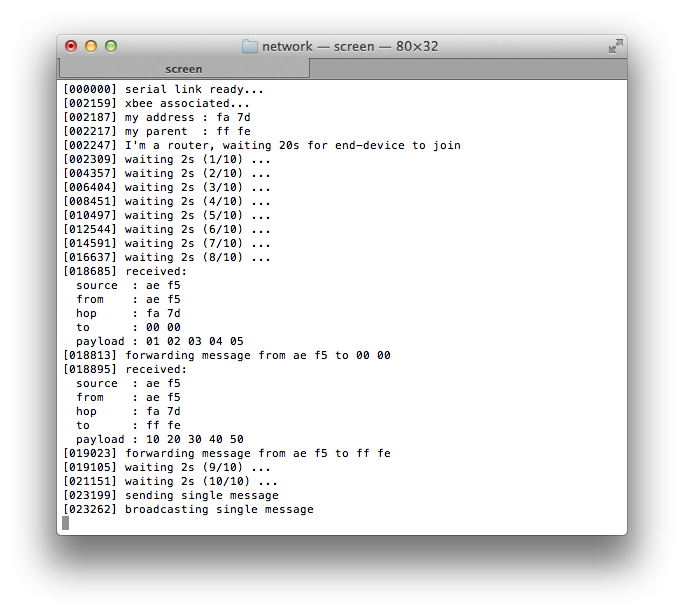
\includegraphics[width=.7\linewidth]{../src/demo/network/router.png}
  \vspace{-3mm}
  \caption{Simulatie van een maasnetwerk: Router}
  \label{fig:virtual-mesh-router}
\end{figure}

\begin{figure}[ht]
  \centering
  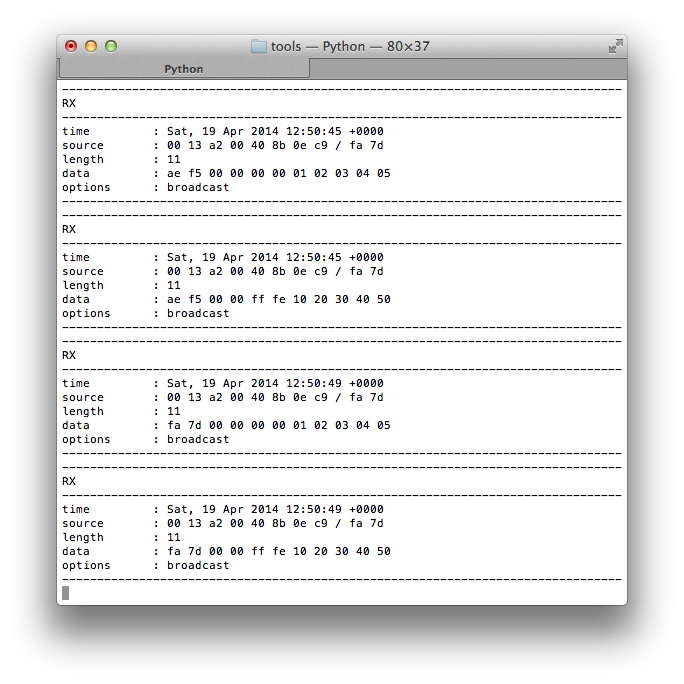
\includegraphics[width=.7\linewidth]{../src/demo/network/coordinator.png}
  \vspace{-3mm}
  \caption{Simulatie van een maasnetwerk: Co\"ordinator}
  \label{fig:virtual-mesh-coordinator}
\end{figure}
